%!TEX root = main.tex
\chapter{Preface}
This thesis was prepared at DTU Compute in fulfillment of the requirements for acquiring an M.Sc. in Digital Media Engineering.
The project has been completed in the period 25th of January to 25th of June and is rated as 30 ECTS points, Associate professor Sune Lehmann Jørgensen has been the supervisor for the project.

The thesis addresses the analysis from and results of datasets for use in a classification problem predicting social ties.

The thesis is structured chronologically and is best read from front to back.

Literature references are given as an ID in index parenthesis [] and can be found in the section Bibliography.
Equations are numbered using X.Y.Z as notation, where X.Y is the section and subsection and Z is the equation number.

%==================================================================================================
% SIGNATURE AREA
%==================================================================================================
\vspace{12mm}
\begin{center}
    \hspace{20mm} Lyngby, \thesishandin-\thesisyear
    \vspace{2mm}
    \newline
  %Update signature image file in line below
    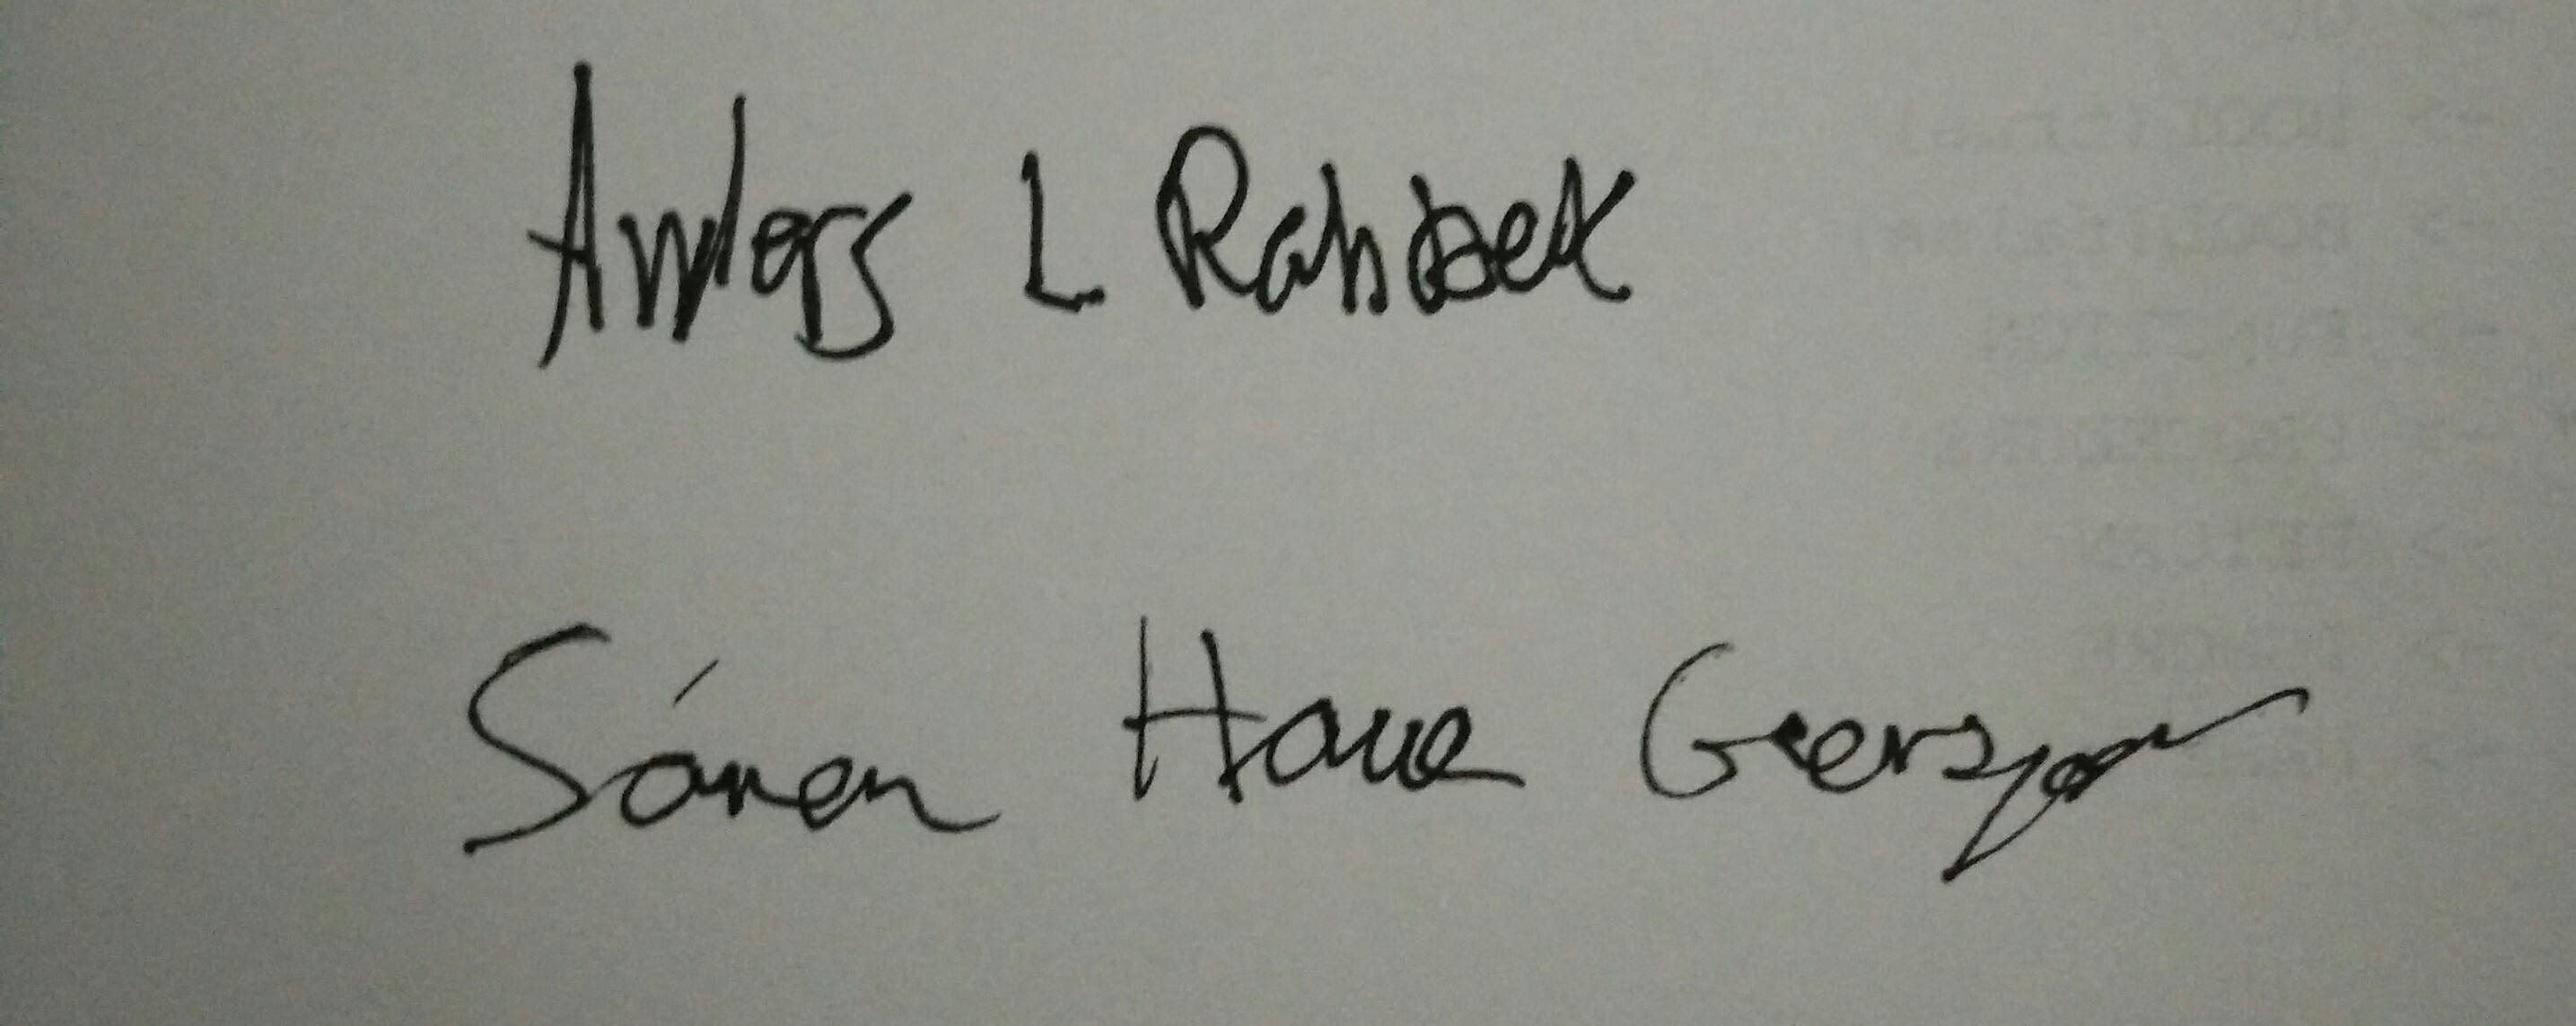
\includegraphics[scale=0.05]{figures/signature}
\end{center}
\begin{flushright}
    \thesisauthor
\end{flushright}
% % % EOF % % %